\chapter[Dubins-Type Trajectory Synthesis Under Terminal Constraints]{Dubins-Type Trajectory Synthesis Under Approach Angle and Arrival Time Constraints\footnote{Some of the theoretical algorithms and formulations in this chapter are derived in part from the author's published work in the \emph{Proceedings of the Mediterranean Conference on Control and Automation (MED) 2024}. This chapter expands upon those preliminary results by providing complete derivations, closed-loop implementation, and comparative lateral acceleration analyses.}}\label{ch:Dubins_Path}
\section{Introduction and Physical Motivation}\label{sec:ch_DP_intro}
In preceding chapters, our investigation focused on distributed multi-agent consensus, establishing exact spectral stability boundaries (Chapter \ref{ch:TwoReverseEdges}), local edge/node scaling remedies (Chapter \ref{ch:Guaranteed_Consensus}), and $\mathcal{H}_2$ performance optimization (Chapter \ref{ch:Robustness_Analysis}). However, executing cooperative team maneuvers in physical environments requires individual autonomous vehicles— such as mobile robots, unmanned aerial vehicles (UAVs), or aerospace interceptors— to execute precise spatial trajectories under nonholonomic kinematic constraints, finite acceleration limits, and specific boundary conditions.

Several guidance and motion planning strategies have emerged in recent years aiming not only to achieve spatial target interception, but also to satisfy simultaneous terminal constraints, such as final impact (approach) angle, terminal time, or both. These dual constraints are critical across various technological applications. For instance, in coordinated robotic manipulation and multi-UAV salvo attacks, controlling the terminal time of arrival guarantees synchronous team convergence. Concurrently, controlling the final approach angle optimizes warhead penetration, aligns sensor fields of view, or avoids defensive countermeasure zones.

Prior literature has extensively explored single-constraint guidance strategies. Target interception under terminal impact angle constraints has been investigated using optimal guidance with time-to-go estimates \cite{zhao2015terminal}, seeker field-of-view constrained guidance \cite{park2013optimal}, biased proportional navigation (BPNG) \cite{kim1998BPNG}, and finite-time sliding mode control \cite{kumar2012sliding}. Similarly, standalone terminal time control has been tackled using feedback linearization \cite{Tekin2016_IT}, Lyapunov-based error dynamics convergence \cite{kim2014lyapunov}, and adaptive sliding mode control \cite{Chen2018_IT}. 

However, achieving \textbf{simultaneous control of both impact angle and terminal time} remains a major practical challenge. Existing dual-constraint methods, such as backstepping protocols \cite{Jung2006}, augmented proportional navigation variants \cite{Zhang2013, Zhang2015}, and multi-mode hybrid switching laws \cite{Harrison2012}, suffer from critical operational drawbacks:
\begin{enumerate}
    \item \textbf{Complex or Discontinuous Acceleration Demands:} They frequently require high-order, continuous time-varying, or infinitely switching (chattering) acceleration profiles that exceed physical actuator bounds ($a_M > a^{\max}$).
    \item \textbf{Inaccurate Time-to-Go Dependencies:} They rely heavily on linear small-angle approximations and time-to-go ($t_{\text{go}}$) estimates that degrade significantly under large heading error angles ($\theta_M \to \pi/2$).
\end{enumerate}

To overcome these limitations, this chapter proposes a computationally efficient, geometrically exact trajectory planning framework utilizing \textbf{Dubins-like path geometry} subject to maximum lateral acceleration bounds ($a^{\max}$). Though the engagement considered in this chapter is a one-on-one scenario (single interceptor against a single target), extensions of this framework to cooperative interception remains a future goal. 

\subsection*{Summary of Key Contributions}
The primary analytical and algorithmic contributions of this chapter are summarized as follows:
\begin{enumerate}
    \item \textbf{Piecewise-Constant Acceleration Profile:} We formulate an open-loop and equivalent closed-loop guidance scheme that requires only three discrete lateral acceleration levels ($+a^{\max}, 0, -a^{\max} \frac{r_m}{r_d}$), eliminating high-order polynomial computation and actuator saturation.
    \item \textbf{Flexible Terminal Time Tuning via Design Radius $r_d$:} Unlike classical Dubins paths \cite{hota2009modified} that utilize two circles of identical minimum turn radius ($r_m = V_M^2 / a^{\max}$) to minimize mission time, we introduce a variable secondary turn radius $r_d \ge r_m$. By adjusting $r_d$, the overall path length (and hence terminal arrival time $t_{\text{imp}}$) may be continuously tuned for any desired approach angle $\theta_t$.
    \item \textbf{Elimination of Feasible Upper Bounds on terminal time via Mirrored Geometry:} We show that when the launch and the approach angles share the same sign, Transverse Common Tangent (TCT) paths have a critical geometric upper bound $r_{\text{crit}}^{\text{TCT}}$. We resolve this limitation by introducing a mirrored TCT circle configuration, rendering the achievable terminal time unbounded above.
    \item \textbf{Singularity-Free Closed-Loop Implementation:} We derive a closed-loop state-feedback implementation governed by distance-to-go switching logic, proving that the guidance law remains non-singular even for large initial heading errors ($\theta_M \approx \pi/2$).
\end{enumerate}

\section{Engagement Kinematics and Problem Formulation}\label{sec:ch_DP_probform}

In this section, we present the mathematical modeling of the two-dimensional interceptor-target engagement scenario and formally state the dual-constraint trajectory planning problem. 

\subsection{Engagement Kinematics and Coordinate System}\label{subsec:ch_DP_kinematics}
Consider the planar engagement geometry depicted in Figure \ref{fig:ch_DP_eng_geometry}, where an autonomous point-mass interceptor pursues a stationary target. The target is located at Cartesian coordinates $(x_T, y_T)$ within an inertial reference frame $\mathcal{F}_I = \{\mathcal{O}; X, Y\}$. Without loss of generality, the origin $\mathcal{O}(0,0)$ is fixed at the interceptor's initial launch position at time $t = 0$.
\begin{figure}[ht!]
	\centering
	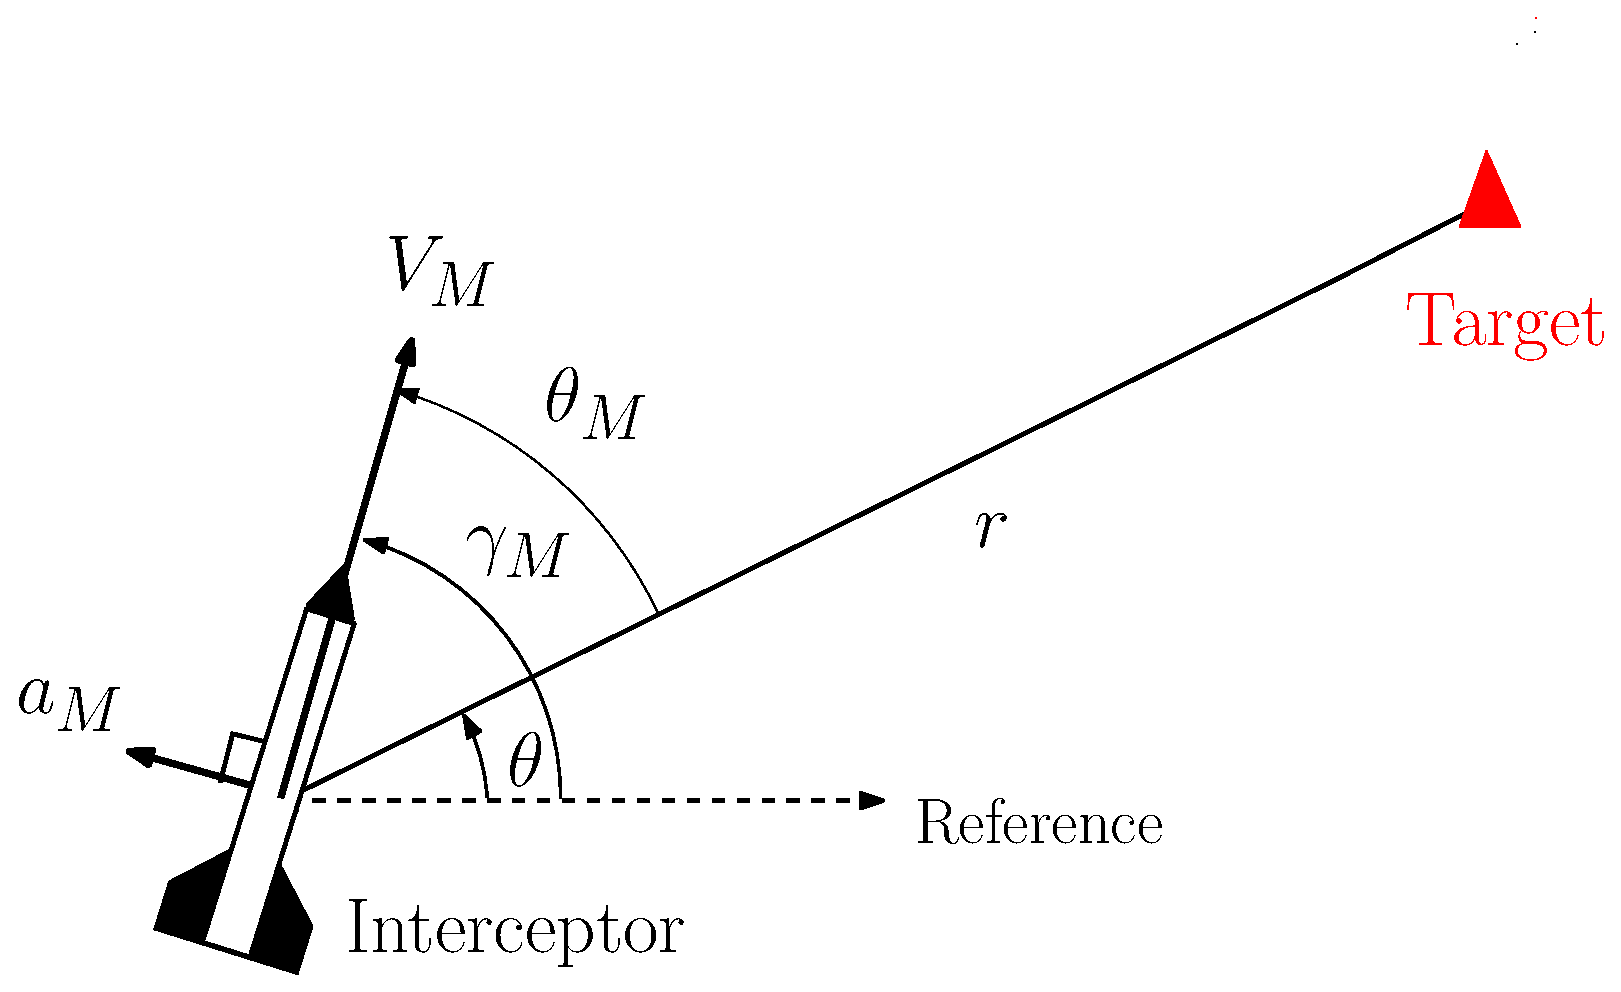
\includegraphics[width=0.8\textwidth, keepaspectratio]{5_Images/dubins_eng.eps}
	\caption{Planar engagement geometry between an autonomous interceptor and a stationary target.}
	\label{fig:ch_DP_eng_geometry}
\end{figure}

Let $(x_M(t), y_M(t))$ denote the position of the interceptor at time $t \ge 0$. The interceptor moves with a constant speed $V_M > 0$, and its instantaneous velocity direction is defined by the flight path angle $\gamma_M(t)$, measured counterclockwise with respect to the global $X$-axis. The control input governing the vehicle's trajectory is the commanded lateral acceleration $a_M(t)$, acting perpendicular to the velocity vector. Consequently, the Cartesian state dynamics of the interceptor are modeled as:
\begin{align}
	\dot{x}_M(t) &= V_M \cos \gamma_M(t), \label{eq:ch_DP_cart_x} \\
	\dot{y}_M(t) &= V_M \sin \gamma_M(t), \label{eq:ch_DP_cart_y} \\
	\dot{\gamma}_M(t) &= \frac{a_M(t)}{V_M}. \label{eq:ch_DP_gamma_dot}
\end{align}

To facilitate guidance law design, the relative kinematics are transformed into polar coordinates $(r, \theta)$, where $r(t)$ denotes the relative range between the interceptor and the target, and $\theta(t)$ denotes the line-of-sight (LOS) angle with respect to the $X$-axis:
\begin{equation}\label{eq:ch_DP_polar_defs}
	r(t) = \sqrt{\big(x_T - x_M(t)\big)^2 + \big(y_T - y_M(t)\big)^2}, \quad \theta(t) = \operatorname{arctan}\Big(y_T - y_M(t), \, x_T - x_M(t)\Big).
\end{equation}

By aligning the initial LOS angle along the horizontal axis ($\theta(0) = 0$), the stationary target's coordinates simplify to $(r(0), 0) = (r_0, 0)$, where $r_0 > 0$ represents the initial range-to-go. The nonholonomic engagement dynamics in polar coordinates are governed by:
\begin{align}
	\dot{r}(t) &= -V_M \cos \theta_M(t), \label{eq:ch_DP_rdot} \\
	r(t) \dot{\theta}(t) &= -V_M \sin \theta_M(t), \label{eq:ch_DP_thetadot}
\end{align}
where $\theta_M(t) \coloneqq \gamma_M(t) - \theta(t)$ represents the lead angle (or look angle) of the interceptor relative to the LOS vector. Equations \eqref{eq:ch_DP_cart_x}--\eqref{eq:ch_DP_thetadot} constitute the complete set of non holonomic kino-dynamic constraints governing planar pursuit.
\subsection{Actuator Limits and Minimum Turn Radius}\label{subsec:ch_DP_actuator_limits}
In practical aerospace and robotic platforms, the commanded lateral acceleration $a_M(t)$ is strictly bounded by structural limits, maximum angle-of-attack thresholds, or motor saturation. We enforce the hard inequality constraint:
\begin{equation}\label{eq:ch_DP_accel_bound}
	|a_M(t)| \le a^{\max}, \quad \forall t \in [0, t_{\text{imp}}],
\end{equation}
where $a^{\max} > 0$ is the maximum allowable lateral acceleration. Substituting constraint \eqref{eq:ch_DP_accel_bound} into kinematic relation \eqref{eq:ch_DP_gamma_dot} establishes a maximum turn rate $\dot{\gamma}_M^{\max} = a^{\max} / V_M$. This physical constraint dictates a fundamental lower bound on the instantaneous radius of curvature of the flight trajectory, termed the minimum turn radius $r_m$:
\begin{equation}\label{eq:ch_DP_min_radius}
	r_m \coloneqq \frac{V_M^2}{a^{\max}}.
\end{equation}
Any admissible geometric path synthesized for the interceptor must possess a local radius of curvature $R(t) \ge r_m$ everywhere along its spatial length.
\subsection{Terminal Constraints and Formal Problem Statement}\label{subsec:ch_DP_problem_statement}
Precision target engagements require enforcing boundary conditions not only on target interception ($r(t_{\text{imp}}) = 0$), but also on the direction of arrival (impact angle) and the total mission time (impact time).
\begin{definition}[Terminal/Impact Time]\label{def:ch_DP_impact_time}
The terminal impact time $t_{\text{imp}} > 0$ is the total elapsed time from interceptor launch ($t = 0$) to target interception ($r(t_{\text{imp}}) = 0$). For a constant flight speed $V_M$, the impact time is directly proportional to the spatial arc length $P$ of the trajectory:
\begin{equation}\label{eq:ch_DP_impact_time_def}
	t_{\text{imp}} = \int_0^{t_{\text{imp}}} \mathrm{d}t = \frac{1}{V_M} \int_0^P \mathrm{d}s = \frac{P}{V_M}.
\end{equation}
\end{definition} 

\begin{definition}[Impact Angle]\label{def:ch_DP_impact_angle}
\leavevmode\par\noindent
The terminal impact angle $\theta_t \in (-\pi, \pi]$ is defined as the orientation of the interceptor's velocity vector relative to the global reference $X$-axis at the precise instant of target interception ($t = t_{\text{imp}}$):
\begin{equation}\label{eq:ch_DP_approach_def}
	\theta_t \coloneqq \lim_{t \to t_{\text{imp}}} \gamma_M(t).
\end{equation}
\end{definition}



With these definitions established, we formally state the dual-constraint trajectory planning problem investigated in this chapter:

\begin{problem}\label{prob:ch_DP_main_problem}
Given an interceptor's initial state vector $\mathbf{x}(0) = [x_M(0), y_M(0), \gamma_M(0)]^T = [0, 0, \gamma_M(0)]^T$, constant speed $V_M$, target initial location $(r_0, 0)$, and maximum lateral acceleration capability $a^{\max}$, synthesize a computationally efficient, singularity-free guidance law $a_M(t)$ such that the following conditions are met:
\begin{enumerate}
    \item \textbf{Target Interception:} The interceptor reaches the target position at time $t = t_{\text{imp}}$, satisfying $r(t_{\text{imp}}) = 0$.
    \item \textbf{Impact Angle Satisfaction:} The velocity vector aligns with the desired approach angle at interception: $\gamma_M(t_{\text{imp}}) = \theta_t$.
    \item \textbf{Impact Time Satisfaction:} Interception occurs exactly at a designated feasible arrival time $t_{\text{imp}} = t^{\star}$.
    \item \textbf{Actuator Feasibility:} The lateral acceleration input satisfies the strict bound $|a_M(t)| \le a^{\max}$ for all $t \in [0, t^{\star}]$.
\end{enumerate}
\end{problem}

\section{Dubins-Like Guidance Path Synthesis}\label{sec:ch_DP_main_design}

In this section, we present the geometric construction of the proposed trajectory planning framework. We first review classic Dubins path theory and discuss its limitations regarding time-of-arrival control, before introducing our variable-radius Dubins-like trajectory architecture.
\subsection{Foundational Principles: Classic Dubins Path Theory and Limitations}\label{subsec:ch_DP_dubins_theory}

The classic path-planning problem formulated by L.E. Dubins (1957) addresses finding the shortest bounded-curvature path between an initial configuration $(x_0, y_0, \theta_0)$ and a final configuration $(x_f, y_f, \theta_f)$ in a two-dimensional Euclidean plane. 

Dubins proved that the optimal trajectory minimizing total path length $P$ belongs to a finite family of paths composed of at most three sequential primitive segments: circular arcs of minimum turn radius $r_m$ (denoted by $L$ for left turn and $R$ for right turn) and straight-line segments (denoted by $S$ for straight). The optimal path family is categorized into two distinct classes:
\begin{enumerate}
    \item \textbf{CSC Class:} Composed of two circular turns connected by a straight line tangent ($\text{LSL}, \text{RSR}, \text{LSR}, \text{RSL}$).
    \item \textbf{CCC Class:} Composed of three consecutive circular turns with alternating directions ($\text{LRL}, \text{RLR}$).
\end{enumerate}

While classic Dubins paths provide time-optimal (shortest-length) trajectories for reaching a target at a specified approach angle, they possess zero flexibility regarding time-of-arrival control. Because all circular arcs in a classic Dubins path are fixed at the minimum radius $r_m$, the total path length $P_{\text{min}}$ is uniquely determined by the initial and final boundary conditions. Consequently, the resulting impact time $t_{\text{imp}}^{\text{min}} = P_{\text{min}} / V_M$ is fixed. If an operational engagement demands a delayed arrival time ($t^{\star} > t_{\text{imp}}^{\text{min}}$) to coordinate salvo strikes or bypass dynamic defenses, classic Dubins paths cannot accommodate the requirement.
\subsection{Proposed Generalized Dubins-Like Path Architecture}\label{subsec:ch_DP_proposed_dubins_concept}

To overcome the temporal rigidity of classic Dubins paths while maintaining bounded acceleration demands ($|a_M(t)| \le a^{\max}$), we generalize the CSC path geometry. Instead of setting both turning radii equal to $r_m$, we assign the radius of the secondary turn circle, centered at the target location as a design parameter.

Specifically, the proposed Dubins-like trajectory consists of three sequential geometric segments:
\begin{enumerate}
	\item \textbf{Primary Circular Arc ($A_1$ on Circle $C_1$):} A turn executed at minimum turn radius $r_m \coloneqq V_M^2 / a^{\max}$ tangential to the interceptor's initial heading vector $\theta_m \coloneqq \theta_M(0)$. This guarantees the fastest initial heading reorientation.
	\item \textbf{Straight Line Tangent ($L_{\text{TCT}}$/$L_{\text{DCT}}$):} A linear segment ($a_M = 0$) directed along the Transverse Common Tangent (TCT) or Direct Common Tangent (DCT) connecting primary circle $C_1$ and secondary circle $C_2$.
	\item \textbf{Secondary Circular Arc ($A_2$ on Circle $C_2$):} A turn executed at a \emph{variable design radius} $r_d \ge r_m$ centered at location $D$, tangential to the target position $(r_0, 0)$ at the desired approach angle $\theta_t$.
\end{enumerate}

By choosing the secondary circle radius $r_d$ as a continuous control design variable ($r_d \in [r_m, r_{\text{crit}}]$), the spatial path length $P(r_d)$ and consequently the terminal arrival time $t_{\text{imp}}(r_d) = P(r_d) / V_M$ becomes a continuously tunable function. Furthermore, enforcing $r_d \ge r_m$ guarantees that the commanded lateral acceleration on circle $C_2$ satisfies:
\begin{equation}\label{eq:ch_DP_rd_accel_bound}
	|a_M|_{C_2} = \frac{V_M^2}{r_d} = a^{\max} \left(\frac{r_m}{r_d}\right) \le a^{\max},
\end{equation}
thereby strictly respecting physical actuator bounds throughout the entire maneuver.

\subsection{TCT Path Geometry with `Same-Sign' Angles}\label{sec:ch_DP_tct_same_sign}
We first analyze the geometric construction when the initial launch angle $\theta_m \in (0, \pi)$ and the terminal approach angle $\theta_t \in (0, \pi)$ share identical algebraic signs (positive counterclockwise orientation relative to the LOS reference), as illustrated in Figure \ref{fig:ch_DP_TCT_samesign}.

\begin{figure}[ht!]
	\centering
	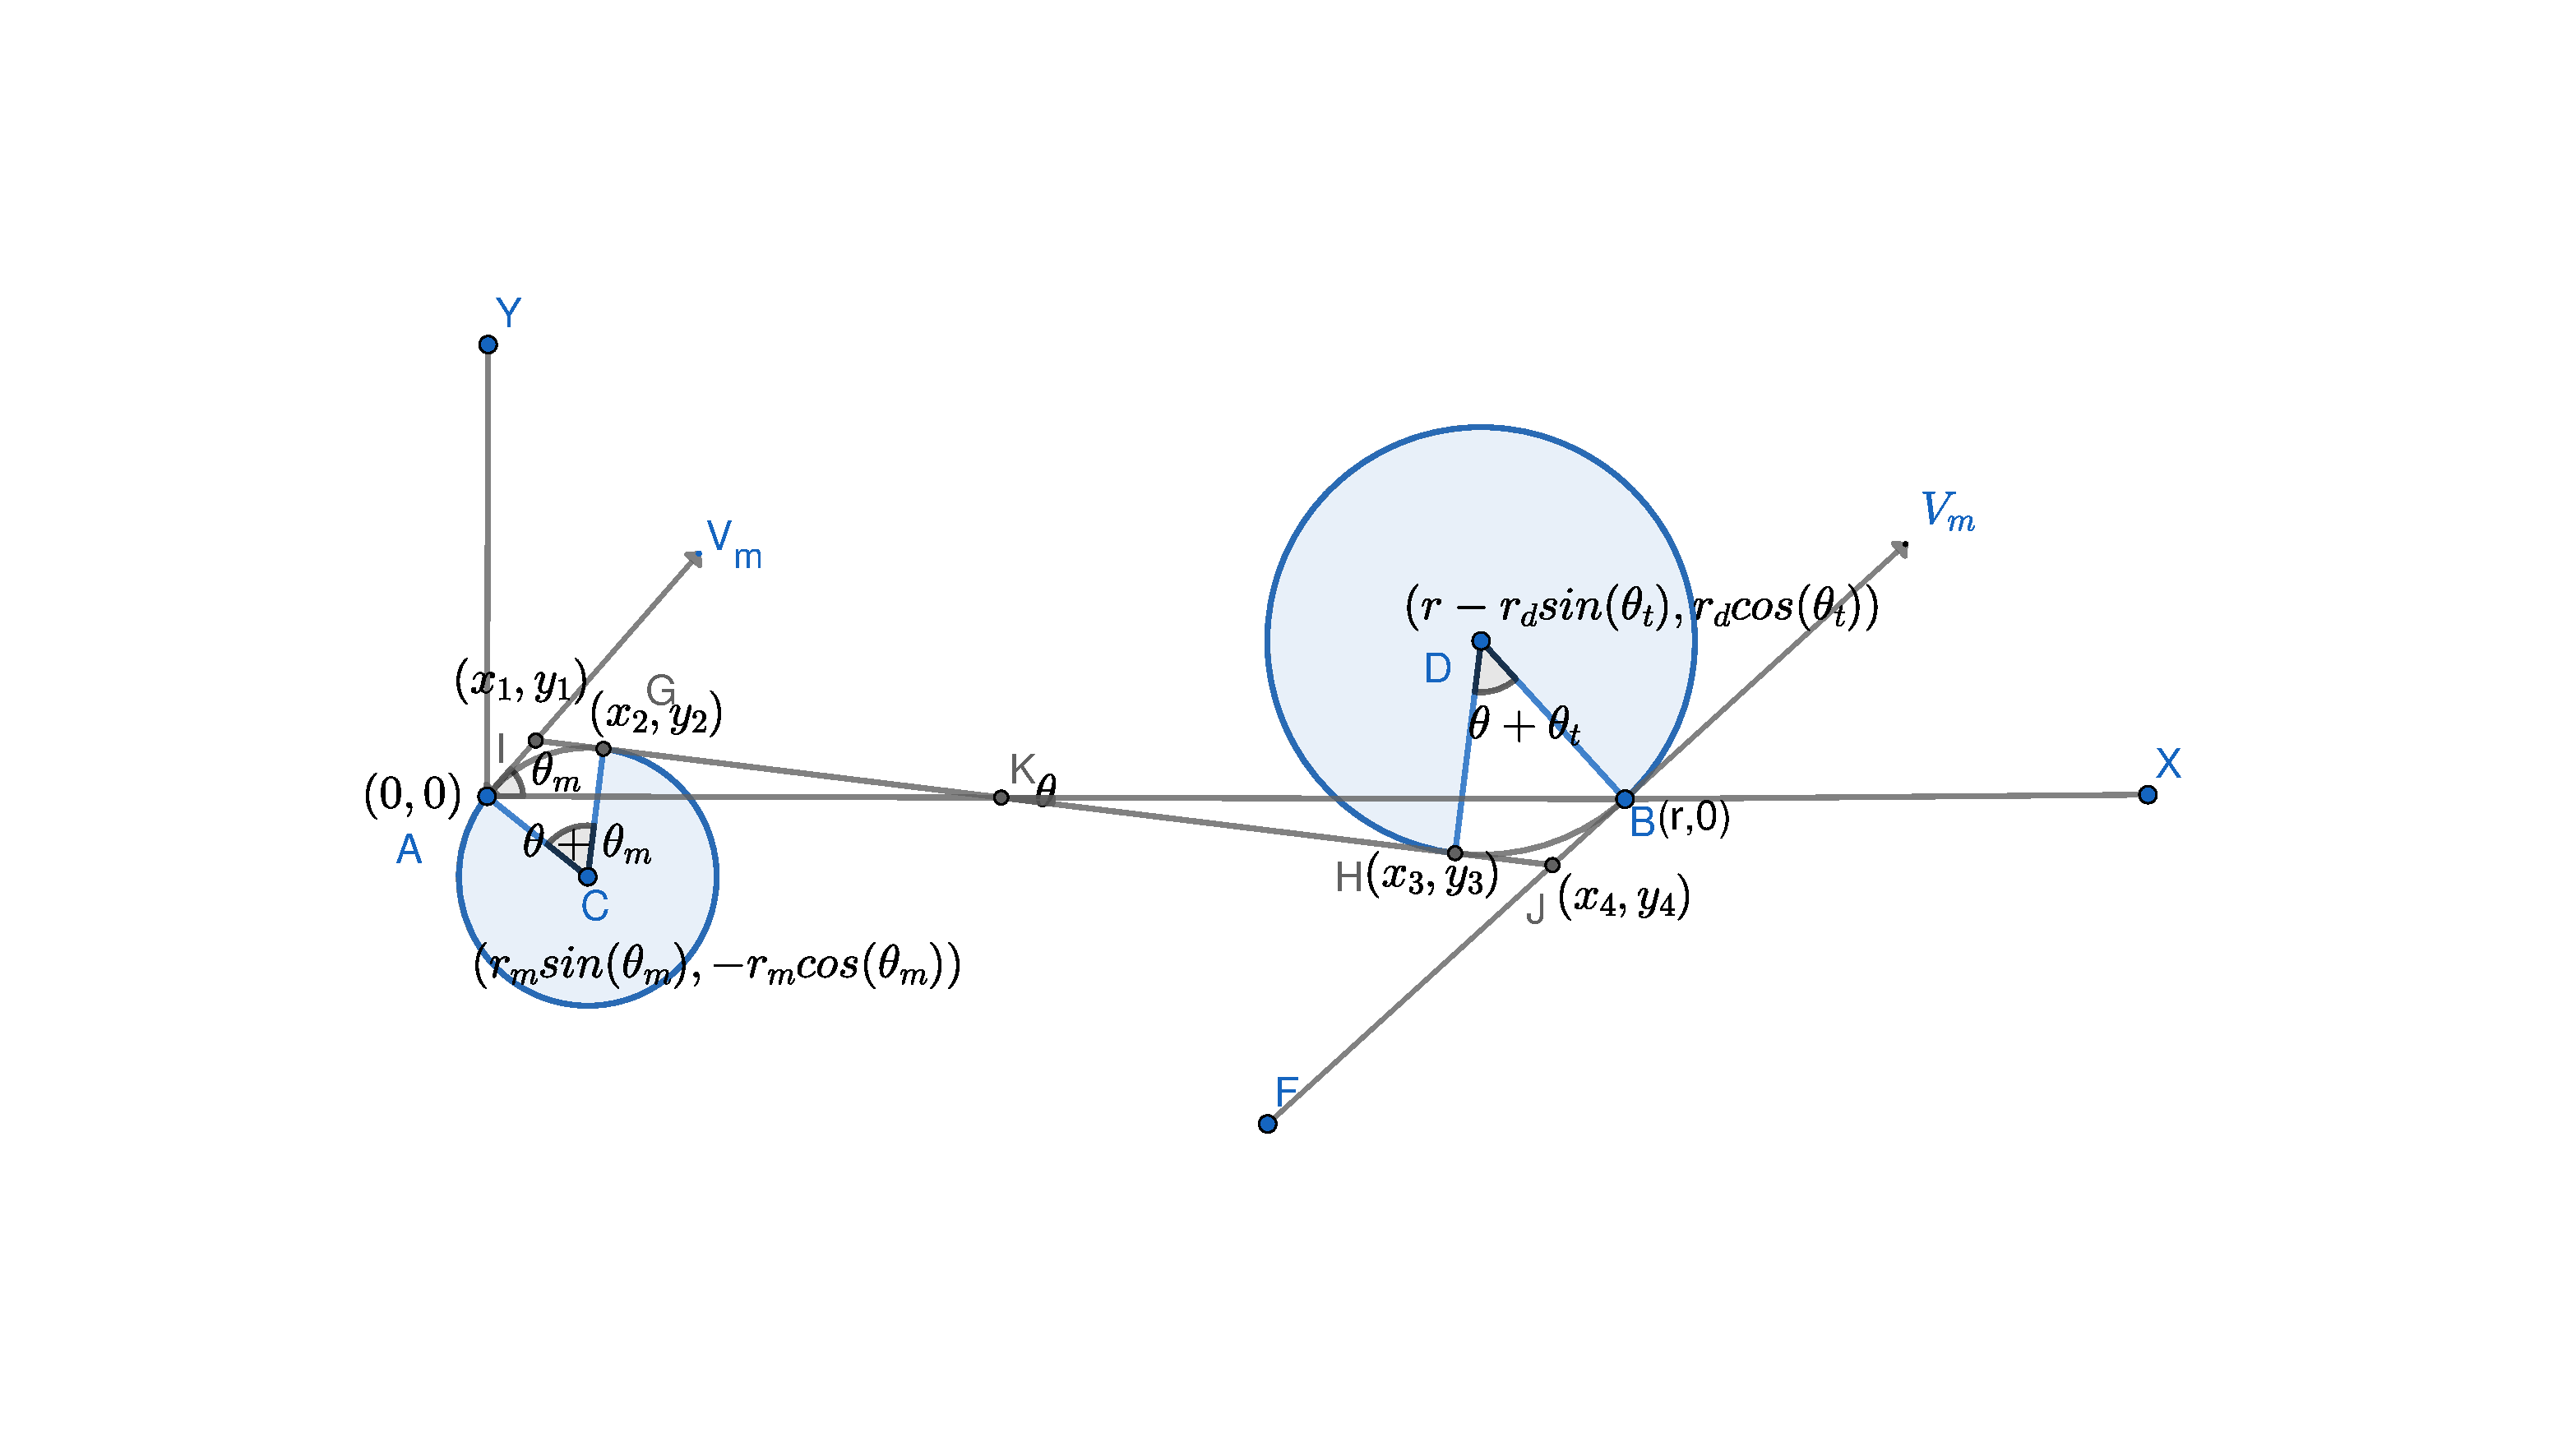
\includegraphics[width=\textwidth, keepaspectratio]{5_Images/TCT_New.pdf}
	\caption{Geometric construction of the TCT Dubins-like path when initial launch angle $\theta_m$ and approach angle $\theta_t$ share the same sign.}
	\label{fig:ch_DP_TCT_samesign}
\end{figure}

The center $C = (x_C, y_C)$ of primary circle $C_1$ and center $D = (x_D, y_D)$ of secondary circle $C_2$ are uniquely determined by vector tangency:
\begin{equation}\label{eq:ch_DP_centers_samesign}
	C = \big(r_m \sin \theta_m, \, -r_m \cos \theta_m\big), \quad D = \big(r - r_d \sin \theta_t, \, r_d \cos \theta_t\big),
\end{equation}
where $r = r_0$ is the initial target range.

The Euclidean distance $d(r_d) \coloneqq \|D - C\|_2$ between circle centers $C$ and $D$ is evaluated using the law of cosines:
\begin{align}\label{eq:ch_DP_center_distance}
	d^2(r_d) &= (r - r_d \sin \theta_t - r_m \sin \theta_m)^2 + (r_d \cos \theta_t + r_m \cos \theta_m)^2 \nonumber \\
	&= r^2 + r_d^2 + r_m^2 + 2 r_d r_m \cos(\theta_m - \theta_t) - 2 r (r_d \sin \theta_t + r_m \sin \theta_m).
\end{align}

For a valid Transverse Common Tangent segment $L_{\text{TCT}}$ to connect circles $C_1$ and $C_2$ externally without overlap, the center-to-center distance must satisfy the geometric condition $d(r_d) \ge r_m + r_d$. As $r_d$ increases, the two circles expand towards each other. The critical upper bound $r_{\text{crit}}^{\text{TCT}}$ occurs at exact circle contact where $d(r_{\text{crit}}^{\text{TCT}}) = r_m + r_{\text{crit}}^{\text{TCT}}$, causing $L_{\text{TCT}} \to 0$:
\begin{equation}\label{eq:ch_DP_rcrit_tct}
	r_{\text{crit}}^{\text{TCT}} = \frac{r^2 - 2 r r_m \sin \theta_m}{2 r_m \left(1 - \cos(\theta_m - \theta_t)\right) + 2 r \sin \theta_t}.
\end{equation}

To compute segment arc lengths, let line $AI$ represent the initial velocity tangent ($y = x \tan \theta_m$), line $BF$ represent the final velocity tangent ($y = (x - r) \tan \theta_t$), and line $IKJ$ denote the TCT segment ($y = -x \tan \theta + c$). Solving the linear intersection systems yields tangent lengths $L_{t1}$ on circle $C_1$ and $L_{t2}$ on circle $C_2$:
\begin{equation}\label{eq:ch_DP_tangent_lengths}
	L_{t1} = \frac{c}{\tan \theta_m + \tan \theta} \sec \theta_m, \quad L_{t2} = \frac{c + r \tan \theta}{\tan \theta_t + \tan \theta} \sec \theta_t,
\end{equation}
where $c = r_m (\cos \theta - \cos \theta_m + \sin \theta \tan \theta + \sin \theta_m \tan \theta)$.

The secondary circle radius $r_d$ relates to $L_{t2}$ via $r_d = L_{t2} \cot \left( \frac{\theta_t + \theta}{2} \right)$. The TCT length $L_{\text{TCT}}$ is obtained by projecting line segments onto the horizontal baseline:
\begin{equation}\label{eq:ch_DP_LTCT_expr}
	L_{\text{TCT}} = \frac{r - L_{t1}(\cos \theta_m + \cos \theta) - L_{t2}(\cos \theta_t + \cos \theta)}{\cos \theta}.
\end{equation}

The total path length $P(r_d)$ for $r_d \in [r_m, r_{\text{crit}}^{\text{TCT}})$ is the sum of the three segment lengths:
\begin{equation}\label{eq:ch_DP_total_path_length}
	P(r_d) = A_1 + L_{\text{TCT}} + A_2 = r_m (\theta_m + \theta) + L_{\text{TCT}} + r_d (\theta_t + \theta),
\end{equation}
and the resulting terminal impact time is $t_{\text{imp}}(r_d) = P(r_d) / V_M$.
\subsection{Mirrored TCT Geometry for Unbounded Arrival Time}\label{sec:ch_DP_tct_mirrored}

While the standard TCT construction in Section \ref{sec:ch_DP_tct_same_sign} allows arrival time tuning, the existence of critical radius $r_{\text{crit}}^{\text{TCT}}$ imposes a upper bound on achievable impact time ($t_{\text{imp}} \le P(r_{\text{crit}}^{\text{TCT}}) / V_M$). When an engagement requires an exceptionally large arrival time, or when the launch angle and approach angle have opposite algebraic signs, circle $C_2$ is mirrored across the target baseline to position $C_2'$, as shown in Figure \ref{fig:ch_DP_TCT_opposite_sign}.

\begin{figure}[ht!]
	\centering
	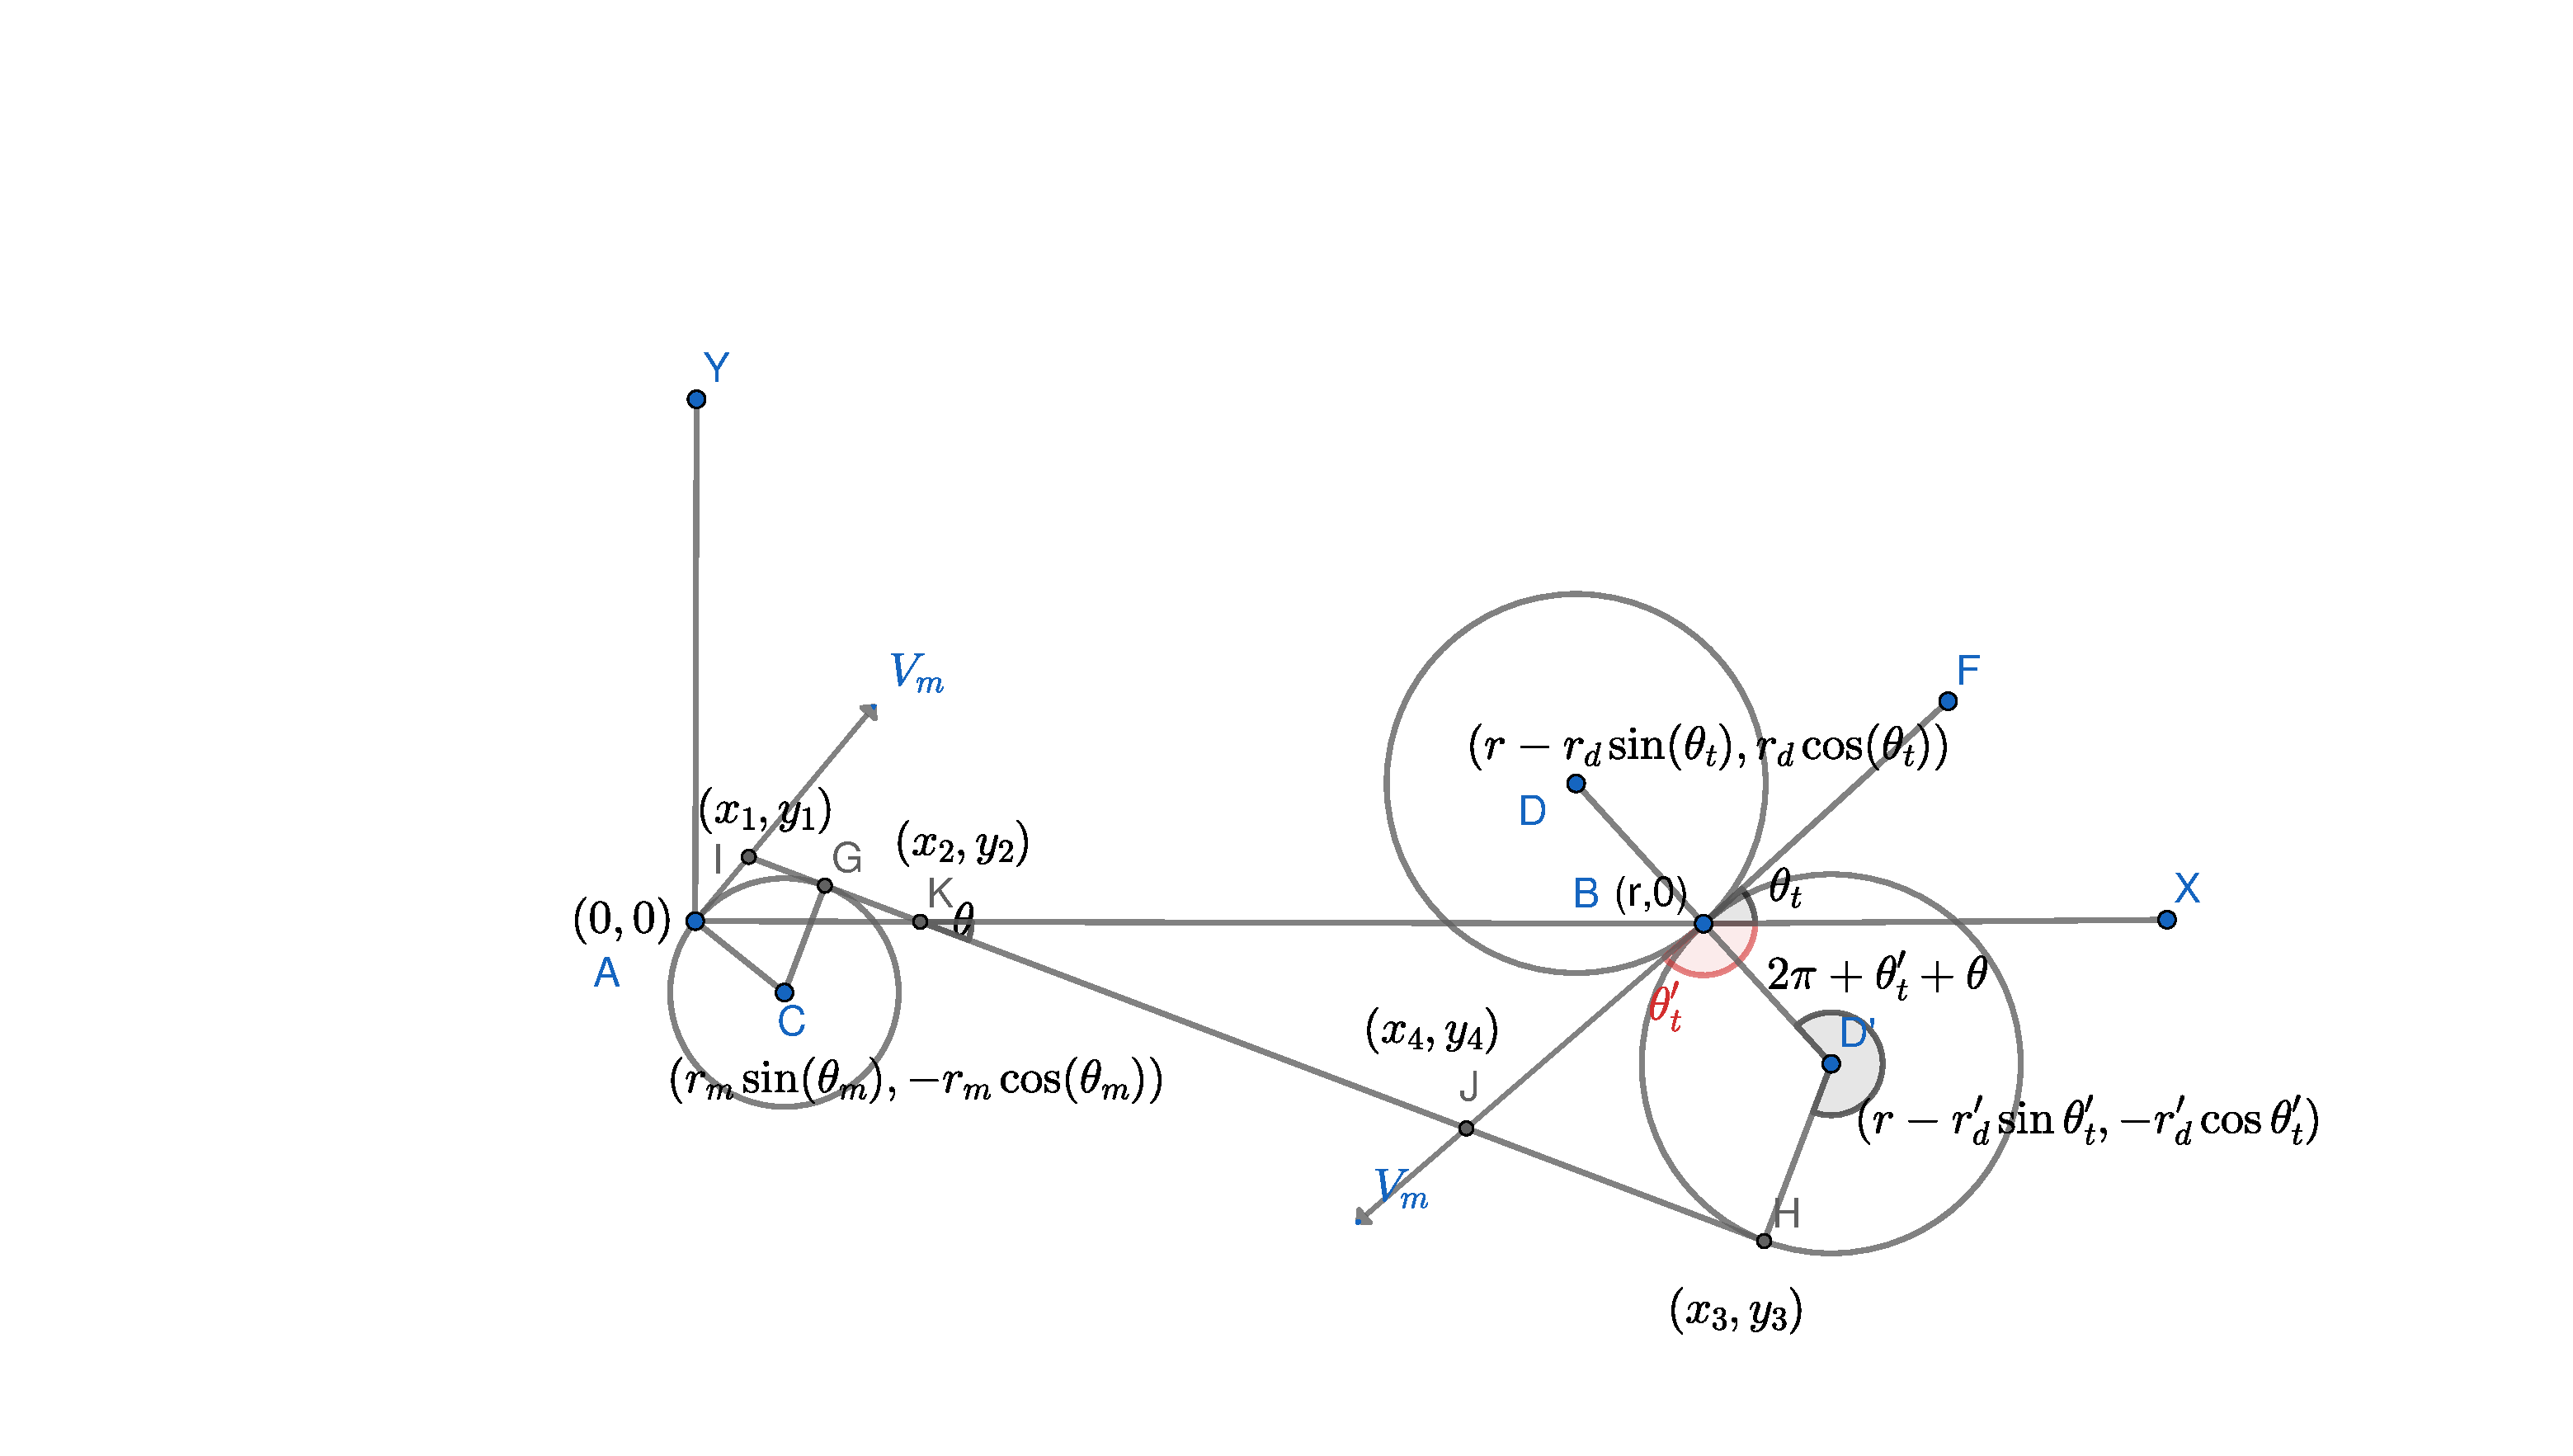
\includegraphics[width=\textwidth, keepaspectratio]{TCTExternal_New.pdf}
	\caption{Mirrored TCT Dubins-like path ($C_2'$), providing unbounded path length $P'(r_d')$ for large terminal time requirements.}
	\label{fig:ch_DP_TCT_opposite_sign}
\end{figure}

The mirrored circle center $D'$ is located at:
\begin{equation}\label{eq:ch_DP_mirrored_center}
	D' = \left( r - r_d' \sin \theta_t', \, -r_d' \cos \theta_t' \right).
\end{equation}

The center-to-center distance $d'(r_d')$ between $C_1$ and $D'$ may be given by:
\begin{equation}\label{eq:ch_DP_mirrored_distance}
	(d')^2 = r^2 + (r_d')^2 + r_m^2 - 2 r_d' r_m \cos(\theta_m + \theta_t') - 2 r (r_d' \sin \theta_t' + r_m \sin \theta_m).
\end{equation}

Because circle $C_2'$ lies on the opposite side of baseline $BF$, $d'(r_d')$ increases monotonically with $r_d'$ without intersecting $C_1$. Consequently, the upper bound constraint is eliminated, rendering the path length $P'(r_d')$ strictly unbounded above ($P' \to \infty$ as $r_d' \to \infty$).

The mirrored arc length traversed on circle $C_2'$ is $A_2' = r_d' (2\pi + \theta_t' + \theta)$, yielding the modified total path length:
\begin{equation}\label{eq:ch_DP_mirrored_path_length}
	P'(r_d') = r_m (\theta_m + \theta) + L_{\text{TCT}}' + r_d' (2\pi + \theta_t' + \theta).
\end{equation}
This mirrored geometry guarantees that any arbitrary, physically feasible impact time $t^{\star} \ge t_{\text{imp}}^{\text{min}}$ can be matched exactly by choosing a suitable radius $r_d'$.

\subsection{Extension to Direct Common Tangent (DCT) and Outer Circle Geometry}\label{subsec:ch_DP_dct_outer}

A geometric constraint of the TCT guidance scheme utilizing an \emph{inner} circle tangential to both launch and target points is the existence of an upper bound on achievable impact time ($t_{\text{imp}} \le P(r_{\text{crit}}^{\text{TCT}}) / V_M$). This bound stems from the critical radius threshold $r_{\text{crit}}^{\text{TCT}}$ at which the two inner circles intersect and the length of the transverse common tangent vanishes ($L_{\text{TCT}} \to 0$).

To overcome this upper bound without requiring vehicle re-orientation or mirrored baseline maneuvers, an alternative construction employs an \emph{outer} circle tangential to the desired velocity vector drawn at the target location, or utilizes a Direct Common Tangent (DCT) configuration. The geometric constructions for TCT and DCT paths with outer circles are depicted in Figure \ref{fig:ch_DP_outer_tct_dct}.

\begin{figure}[!ht]
	\centering
	\begin{subfigure}[b]{0.7\textwidth}
		\centering
		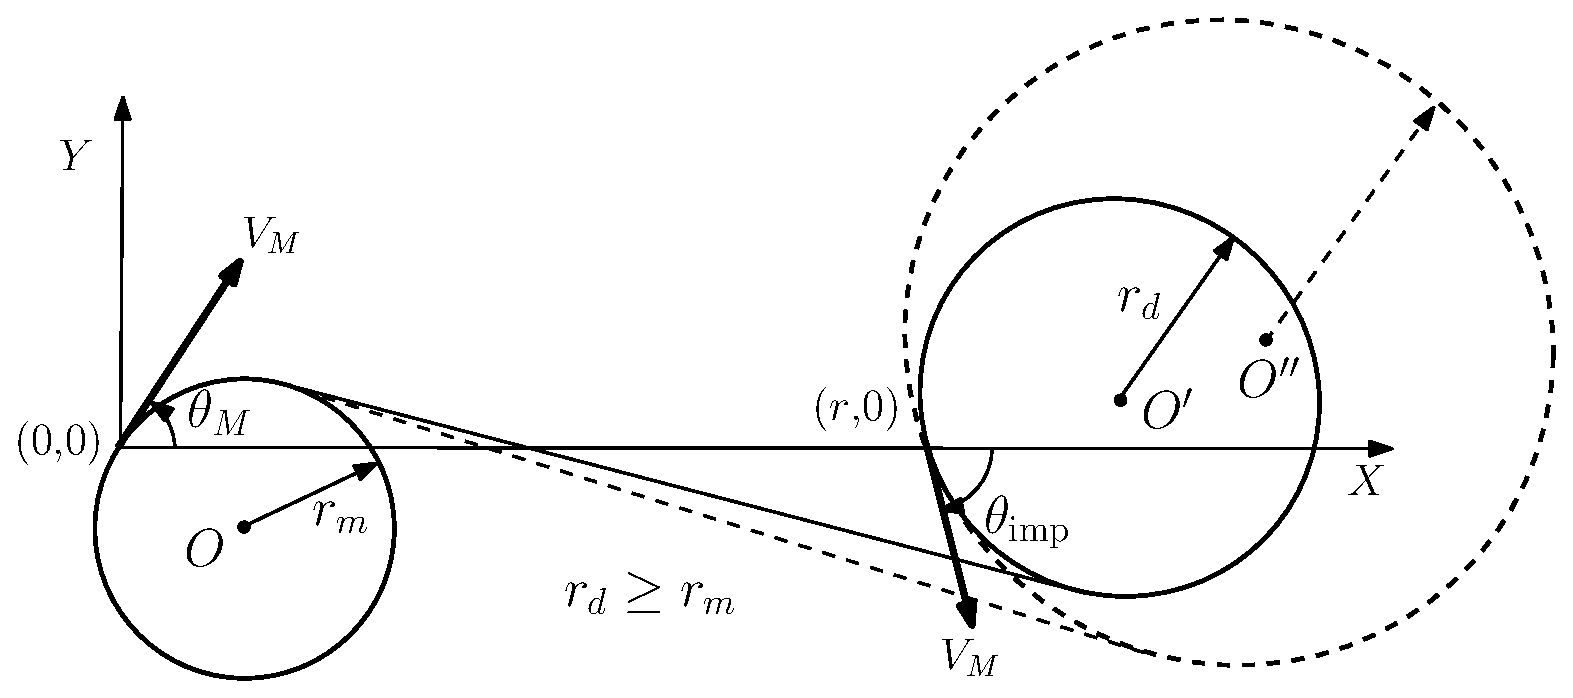
\includegraphics[width=\textwidth]{fig44.eps}
		\caption{Transverse common tangent (TCT) path.}
		\label{fig:ch_DP_figtct}
	\end{subfigure}
	\hfill
	\begin{subfigure}[b]{0.7\textwidth}
		\centering
		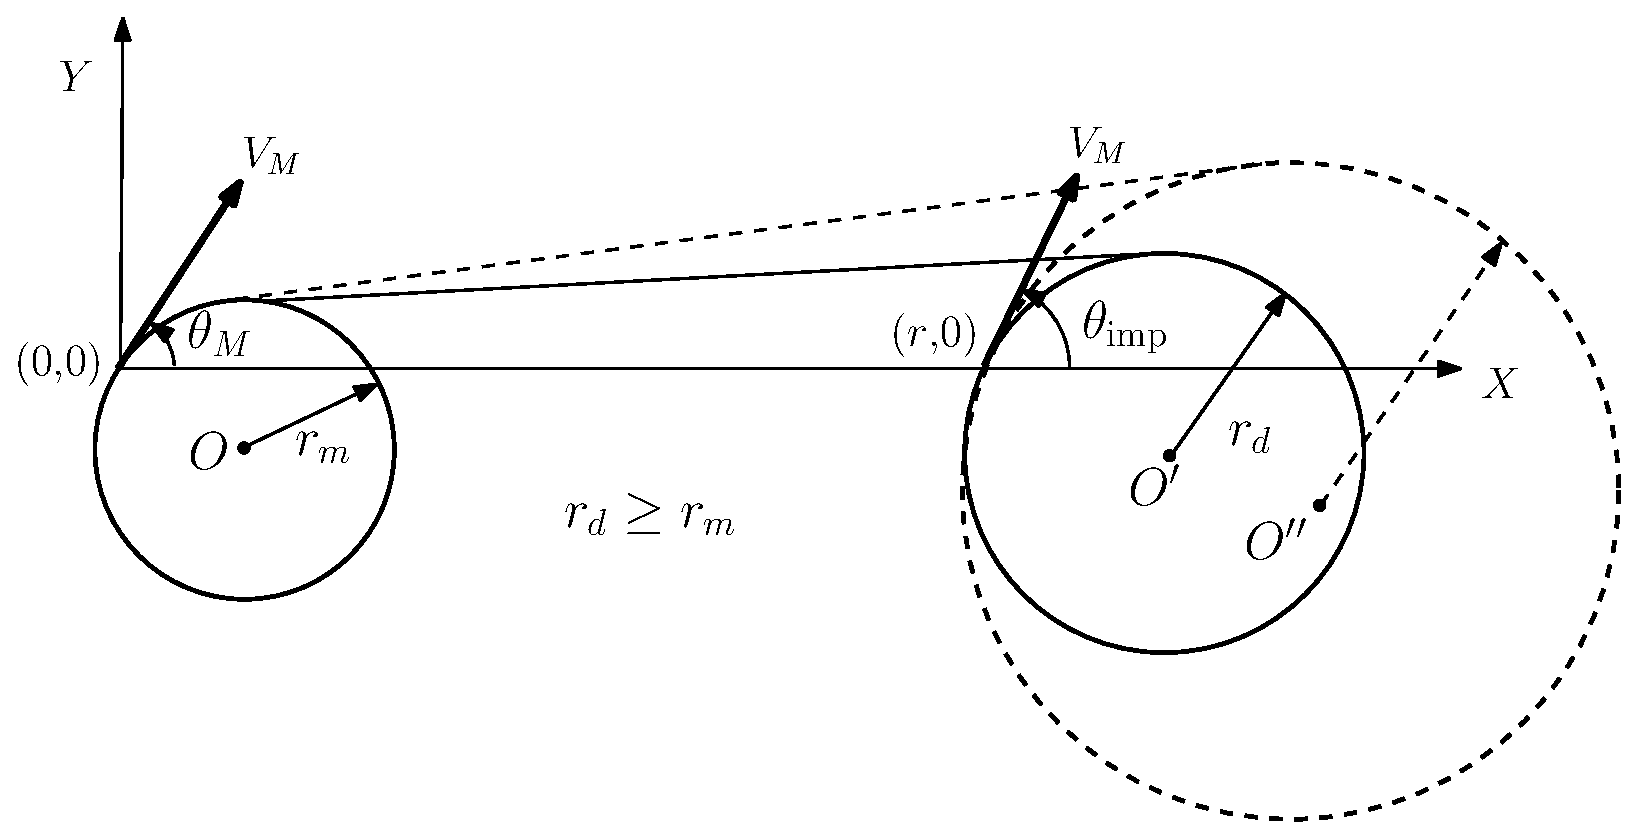
\includegraphics[width=\textwidth]{fig33.eps}
		\caption{Direct common tangent (DCT) path.}
		\label{fig:ch_DP_figdct}
	\end{subfigure}
	\caption{Dubins-like path geometry utilizing an \emph{outer} circle at the target location to satisfy simultaneous impact angle and unbounded impact time requirements.}
	\label{fig:ch_DP_outer_tct_dct}
\end{figure}

The primary geometric distinctions between TCT and DCT outer configurations are characterized by the velocity vector alignments along the vertical axis:
\begin{itemize}
    \item \textbf{Transverse Common Tangent (TCT):} Corresponds to engagement geometries where the $Y$-components of the interceptor's initial and final velocity vectors have \emph{opposite algebraic signs} ($\operatorname{sgn}(V_{y,0}) \neq \operatorname{sgn}(V_{y,f})$).
    \item \textbf{Direct Common Tangent (DCT):} Corresponds to engagement geometries where the initial and final velocity vectors lie in the same vertical half-plane ($\operatorname{sgn}(V_{y,0}) = \operatorname{sgn}(V_{y,f})$), i.e., both velocity vectors have positive $Y$-components (quadrants I and II) or both have negative $Y$-components (quadrants III and IV).
\end{itemize}

As evident from Figure \ref{fig:ch_DP_outer_tct_dct}, placing an outer circle at the target location eliminates circle-intersection limits. Consequently, no finite upper bound exists for the secondary radius ($r_d \in [r_m, \infty)$). As $r_d \to \infty$, the total path length increases continuously ($P(r_d) \to \infty$), allowing exact matching for arbitrarily large desired impact time values, $t^{\star}$.

Importantly, the fundamental structure of the lateral acceleration guidance command in \eqref{eq:ch_DP_open_loop_guidance} and its closed-loop state feedback counterpart in \eqref{eq:ch_DP_closed_loop_guidance} remain \emph{identical}. The piecewise-constant control command continues to demand exactly three discrete acceleration levels ($+a^{\max}, 0, -a^{\max}\frac{r_m}{r_d}$), provided that the design radius $r_d$ and switching lengths ($A_1, L_{\text{DCT}}, A_2$) are evaluated using the corresponding DCT/outer-circle geometric equations.
\subsection{Path Length Monotonicity}\label{subsec:ch_DP_monotonicity}

The fundamental property that enables precise numerical root-finding (such as bisection or Newton-Raphson methods) to obtain $r_d$ for a desired target impact time $t^\star$ is the monotonicity of the path length functions.

\begin{remark}[Path Length Monotonicity]\label{rem:ch_DP_monotonicity}
The path length $P(r_d)$ defined in \eqref{eq:ch_DP_total_path_length} is a strictly monotonically increasing function of $r_d$ over the interval $r_d \in [r_m, r_{\text{crit}}^{\text{TCT}}]$. Similarly, the mirrored path length $P'(r_d')$ defined in \eqref{eq:ch_DP_mirrored_path_length} is a strictly monotonically increasing function over $r_d' \in [r_m, \infty)$.
\end{remark}

The variation of total path length $P$ with respect to the designed turning radius $r_d$ for the TCT-based formulation is illustrated in Figure \ref{fig:ch_DP_lengthvsradius}.

\begin{figure}[!ht]
	\centering
	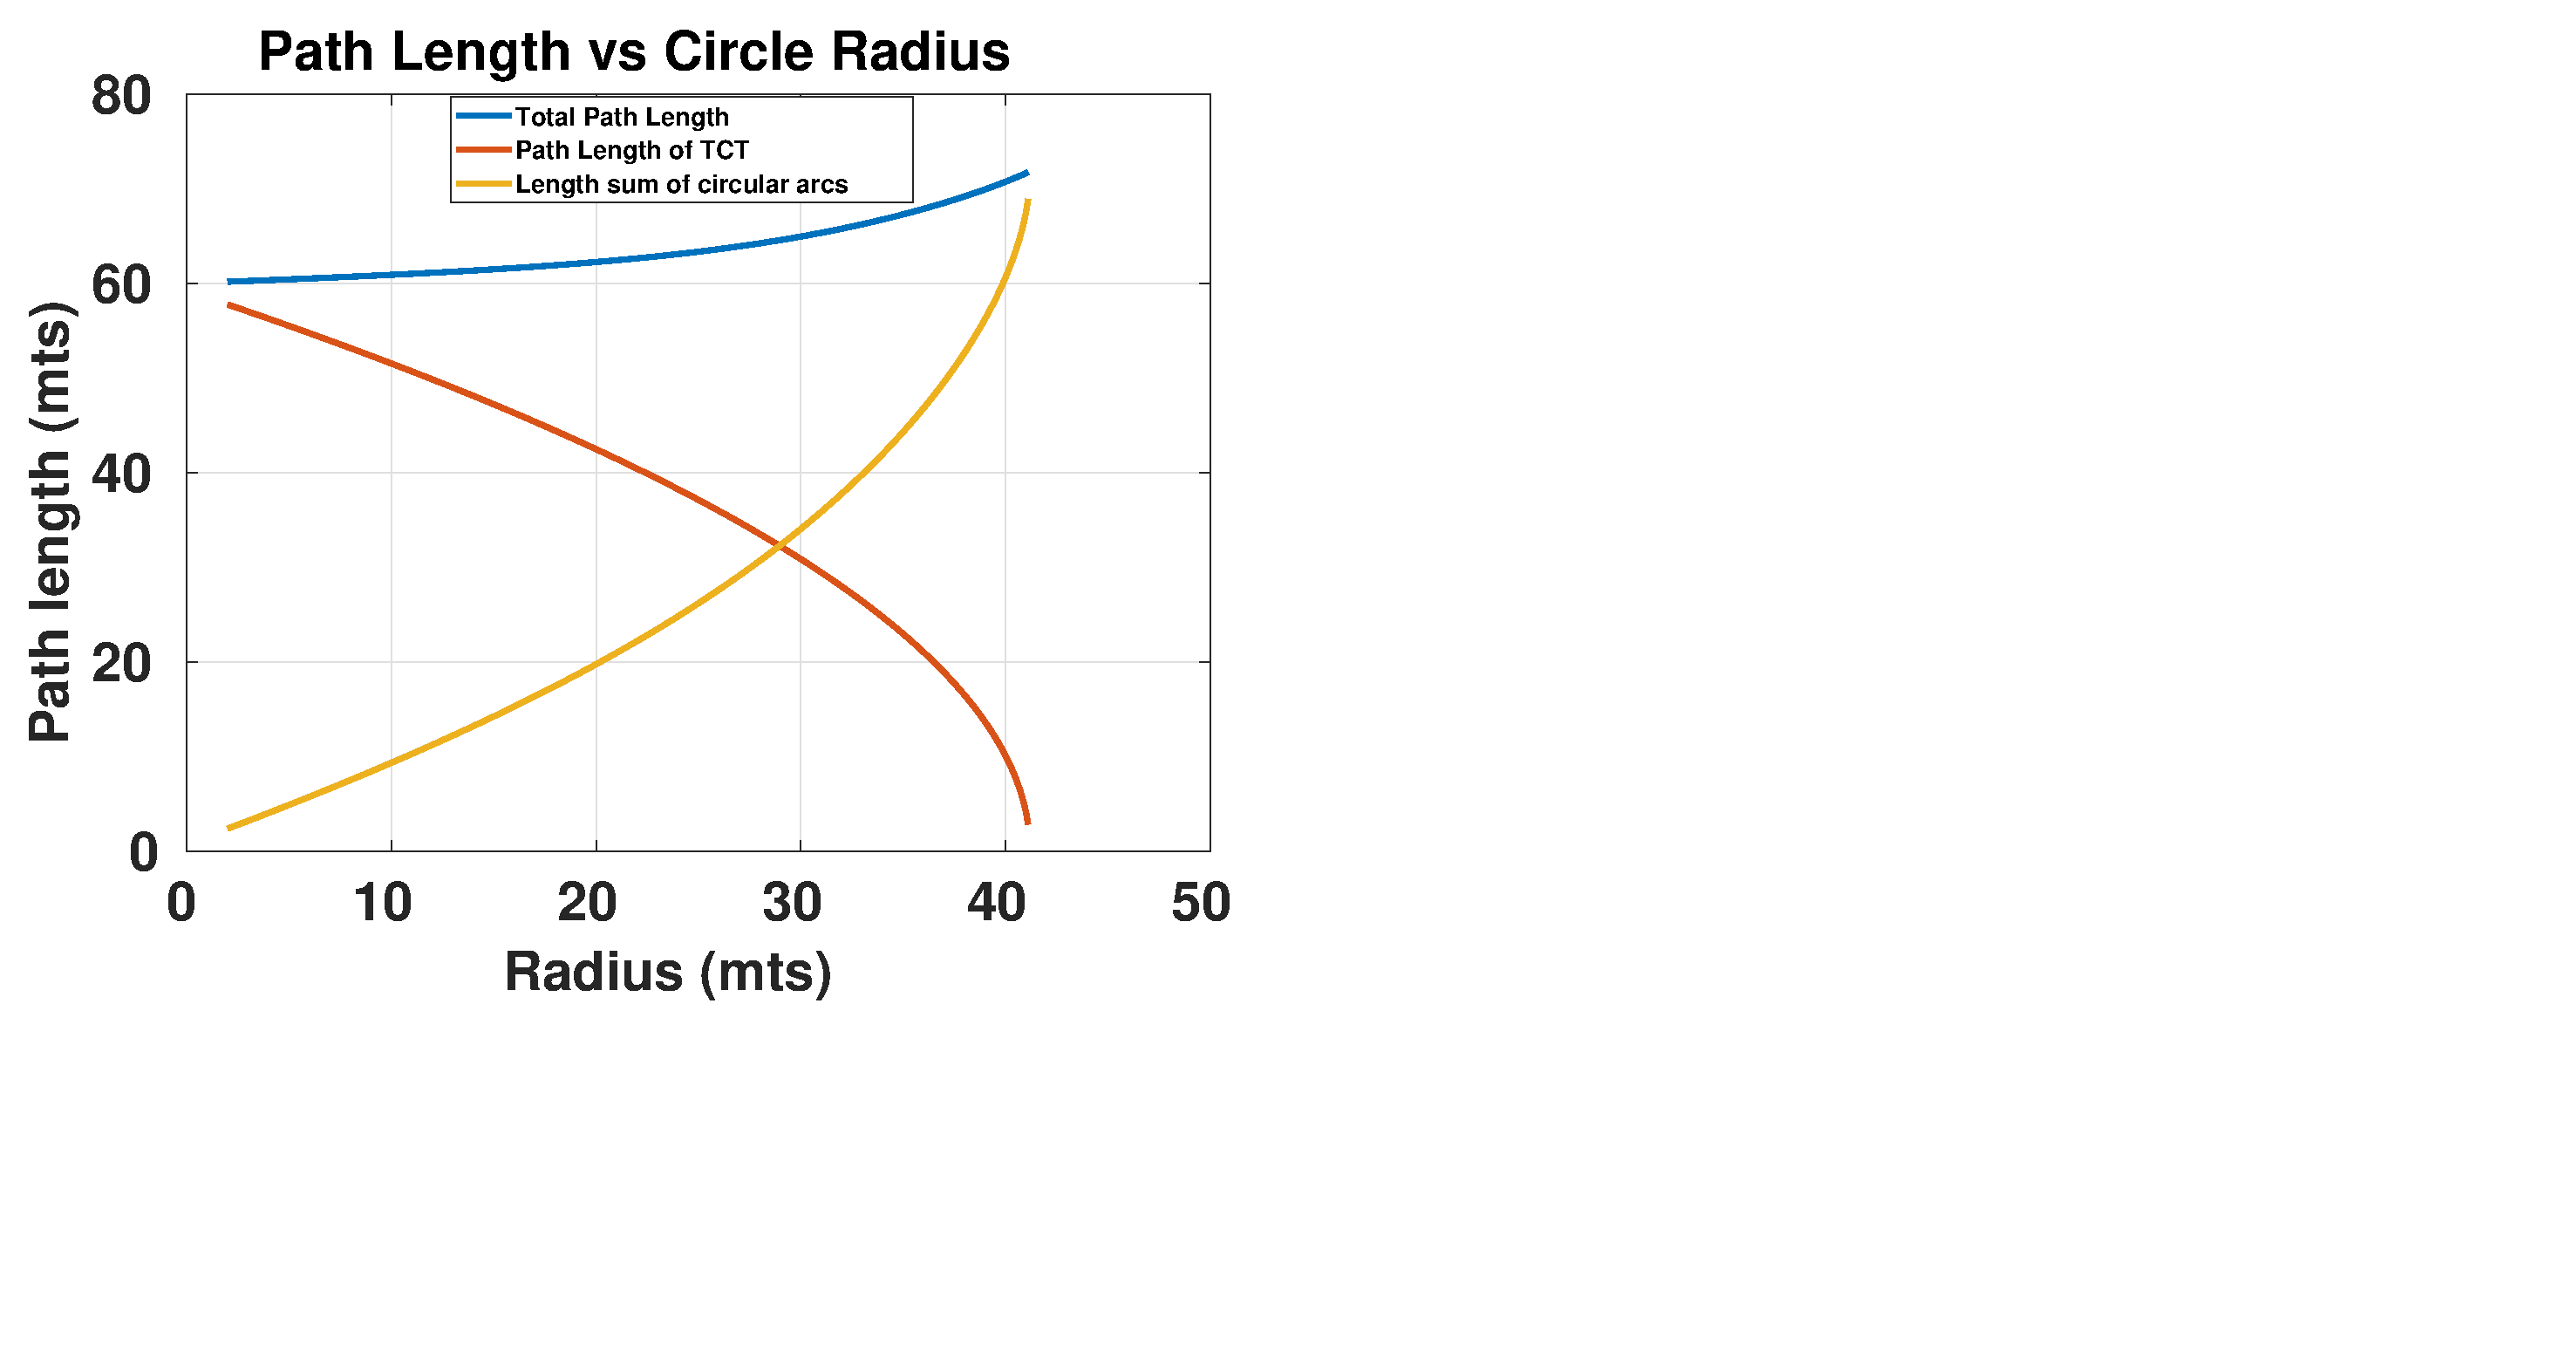
\includegraphics[trim={0cm 6cm 25cm 0cm},clip,scale=0.6]{5_Images/RadiusVsPathLength1.eps}
	\caption{Path length variation versus secondary turning radius $r_d \in [r_m, r_{\text{crit}}^{\text{TCT}})$.}
	\label{fig:ch_DP_lengthvsradius}
\end{figure}

Because $P(r_d)$ and $P'(r_d')$ are strictly monotonic and continuous, by the Intermediate Value Theorem \cite{rudin1964principles}, for any desired arrival time $t^\star \in [t_{\text{imp}}(r_m), t_{\text{imp}}(r_{\text{crit}}))$, there exists a unique secondary radius $r_d^\star$ satisfying $t_{\text{imp}}(r_d^\star) = t^\star$.
\section{Guidance Protocol and Implementation}\label{sec:ch_DP_guidance_law}
In Section \ref{sec:ch_DP_main_design}, we established the static spatial geometry of the Dubins-like path, determining the exact arc lengths $A_1$, $A_2$, common tangent length $L_{\text{TCT}}$, and secondary turning radius $r_d$ required to achieve the desired terminal approach angle $\theta_t$ and arrival time $t^{\star}$. However, physically executing this spatial trajectory requires converting static geometric parameters into a time-varying lateral acceleration command $a_M(t)$ that the autopilot can track dynamically.

In this section, we construct the open-loop guidance protocol and subsequently reformulate it into a robust, singularity-free closed-loop state feedback law.
\subsection{Mapping Spatial Geometry to Temporal Acceleration Demands}\label{subsec:ch_DP_spatial_to_temporal}

Because the interceptor operates at a constant forward velocity $V_M$, there exists a direct linear mapping between spatial progress along the path (arc length $s$) and temporal elapsed time ($t = s / V_M$). Each of the three distinct path segments synthesized in Section \ref{sec:ch_DP_main_design} corresponds to a dedicated time interval during which a constant lateral acceleration command is applied:

\begin{enumerate}
    \item \textbf{Phase 1: Initial Turning Segment ($0 \le t < t_1$):} To traverse arc $A_1$ on primary circle $C_1$ at minimum turn radius $r_m = V_M^2 / a^{\max}$, the interceptor demands maximum lateral acceleration:
    \begin{equation}\label{eq:ch_DP_phase1_accel}
        |a_M(t)| = \frac{V_M^2}{r_m} = a^{\max}.
    \end{equation}
    The duration of this initial reorientation phase is strictly given by $t_1 = A_1 / V_M$.
    
    \item \textbf{Phase 2: Straight-Line Cruise Segment ($t_1 \le t < t_1 + t_2$):} Along the Transverse Common Tangent $L_{\text{TCT}}$, the path curvature is zero ($\kappa = 0$). Consequently, the guidance command vanishes:
    \begin{equation}\label{eq:ch_DP_phase2_accel}
        a_M(t) = 0.
    \end{equation}
    The elapsed time spent along the straight tangent is $t_2 = L_{\text{TCT}} / V_M$.
    
    \item \textbf{Phase 3: Terminal Alignment Segment ($t_1 + t_2 \le t \le t_{\text{imp}}$):} To traverse arc $A_2$ on secondary circle $C_2$ at design radius $r_d$, the vehicle demands a reduced lateral acceleration:
    \begin{equation}\label{eq:ch_DP_phase3_accel}
        |a_M(t)| = \frac{V_M^2}{r_d} = a^{\max} \left( \frac{r_m}{r_d} \right) \le a^{\max}.
    \end{equation}
    The duration of this final turn is $t_3 = A_2 / V_M$, yielding the total time of flight $t_{\text{imp}} = t_1 + t_2 + t_3$.
\end{enumerate}
\subsection{Piecewise-Constant Open-Loop Guidance Command}\label{subsec:ch_DP_open_loop}

Combining the three temporal phases described in Section \ref{subsec:ch_DP_spatial_to_temporal}, the demanded lateral acceleration $a_M(t)$ is generated as a piecewise-constant function governed by two discrete switching instants:
\begin{equation}\label{eq:ch_DP_open_loop_guidance}
	a_M(t) = \begin{cases}
		a^{\max} \operatorname{sgn}(x), & \text{for } 0 \le t < t_1, \\
		0, & \text{for } t_1 \le t < t_1 + t_2, \\
		a^{\max} \left( \frac{r_m}{r_d} \right) \operatorname{sgn}(y), & \text{for } t_1 + t_2 \le t \le t_{\text{imp}},
	\end{cases}
\end{equation}
where $t_1 = A_1 / V_M$, $t_2 = L_{\text{TCT}} / V_M$, and $t_3 = A_2 / V_M$ (such that $t_{\text{imp}} = t_1 + t_2 + t_3$), $\operatorname{sgn}(\cdot)$ is the standard signum function, and $x, y \in \mathbb{R} \setminus \{0\}$ establish turn directionalities (clockwise versus counterclockwise) depending on whether a standard or mirrored TCT geometry is selected.

\begin{remark}[Actuator Feasibility and Energy Efficiency]\label{rem:ch_DP_acceleration_efficiency}
Because the secondary turn radius is constrained by $r_d \ge r_m$, the terminal acceleration magnitude strictly satisfies $|a_M(t)| = a^{\max} \frac{r_m}{r_d} \le a^{\max}$. The total $L_1$-norm acceleration energy expenditure across the engagement is:
\begin{equation}\label{eq:ch_DP_acceleration_energy}
	\|a_M\|_1 \coloneqq \int_0^{t_{\text{imp}}} |a_M(t)| \mathrm{d}t = \left( \frac{r_d t_1 + r_m t_3}{r_d} \right) a^{\max},
\end{equation}
yielding an average lateral acceleration requirement of $\bar{a}_M = \left( \frac{r_d t_1 + r_m t_3}{r_d t_{\text{imp}}} \right) a^{\max} < a^{\max}$, which is significantly lower than classical high-gain terminal guidance laws.
\end{remark}
\subsection{Singularity-Free Closed-Loop Feedback Implementation}\label{subsec:ch_DP_closed_loop}

While the open-loop guidance law \eqref{eq:ch_DP_open_loop_guidance} mathematically satisfies all boundary conditions in ideal simulation environments, pure open-loop execution is highly sensitive to external wind disturbances, target position uncertainty, and autopilot response lag. To provide robust tracking capability, open-loop law \eqref{eq:ch_DP_open_loop_guidance} is reformulated into a closed-loop feedback structure.

Rather than indexing control switches by elapsed time $t$ (which accumulates clock drift), the closed-loop feedback law is driven by the instantaneous cumulative arc length $S(t)$ traversed by the interceptor from its states:
\begin{equation}\label{eq:ch_DP_arc_length_state}
    S(t) \coloneqq \int_0^t V_M(\tau) \mathrm{d}\tau = \int_0^t \sqrt{\dot{x}_M^2(\tau) + \dot{y}_M^2(\tau)} \, \mathrm{d}\tau.
\end{equation}

Using arc-length progress $S(t)$ as the feedback metric, the closed-loop guidance protocol is formulated as:
\begin{equation}\label{eq:ch_DP_closed_loop_guidance}
	a_M(S) = \frac{a^{\max}}{2} \left[ \left( 1 + \operatorname{sgn}(A_1 - S) \right) \operatorname{sgn}(x) + \left( \frac{r_m}{r_d} \right) \left( 1 - \operatorname{sgn}(A_1 + L_{\text{TCT}} - S) \right) \operatorname{sgn}(y) \right].
\end{equation}

To eliminate high-frequency control chattering and actuator wear across the switching boundaries $S = A_1$ and $S = A_1 + L_{\text{TCT}}$, the discontinuous signum functions in \eqref{eq:ch_DP_closed_loop_guidance} are approximated using hyperbolic tangent smoothers:
\begin{equation}\label{eq:ch_DP_sigmoid_smoothing}
	\operatorname{sgn}(\Delta S) \approx \tanh\left( \frac{\Delta S}{\epsilon_b} \right),
\end{equation}
where $\epsilon_b > 0$ denotes a small user-defined boundary layer width governing transition smoothness.

\begin{remark}[Singularity Avoidance at High Heading Errors]\label{rem:ch_DP_singularity_free}
\leavevmode\par\noindent
Conventional impact-time guidance laws (such as \cite{harl2011impact}) contain $\sec \theta_M$ terms that singularize when the lead angle approaches $\pi/2$ ($\theta_M \approx 90^\circ$). Because protocol \eqref{eq:ch_DP_closed_loop_guidance} relies on global arc-length progress $S(t)$ rather than LOS rate division, it is completely singularity-free for all launch angles $\theta_M(0) \in (-\pi, \pi]$.
\end{remark}

\section{Numerical Simulation Results}\label{sec:ch_DP_simulations}
Numerical simulations were performed to evaluate the guidance framework under various engagement geometries. The interceptor operates at constant speed $V_M = 500\text{ m/s}$ with maximum acceleration capacity $a^{\max} = 400\text{ m/s}^2$ ($r_m = 625\text{ m}$). The initial range to the stationary target is $r(0) = 10,000\text{ m}$.

\subsection{Simultaneous Impact Angle and Time Control}

In the first test scenario, the initial heading angle is set to $\gamma_M(0) = 90^\circ$ ($\theta_M(0) = 90^\circ$), with desired approach angle $\theta_t = 45^\circ$ and required arrival time $t^{\star} = 22.0\text{ s}$. 

Solving $t_{\text{imp}}(r_d) = 22.0\text{ s}$ yields design radius $r_d = 4,400\text{ m}$, giving segment times $[t_1, t_2, t_3] = [2.389, 9.729, 9.909]\text{ s}$. Figures \ref{fig:ch_DP_sim1_trajs} and \ref{fig:ch_DP_sim1_accel} display the trajectory and smooth piecewise-constant lateral acceleration profile $a_M(t)$. The interceptor hits the target at exactly $t = 22.0\text{ s}$ with terminal angle $\gamma_M(t_{\text{imp}}) = 45.0^\circ$.

\begin{figure}[ht!]
	\centering
	\begin{subfigure}[b]{0.8\textwidth}
		\centering
		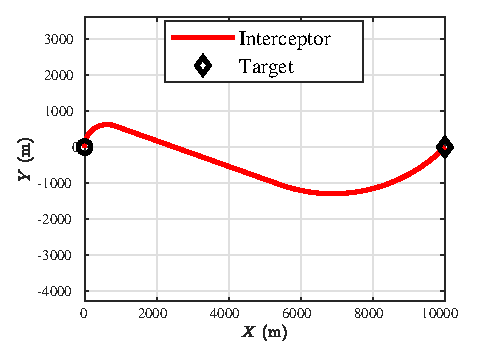
\includegraphics[width=\textwidth, keepaspectratio]{5_Images/trajakd.eps}
		\caption{Spatial engagement trajectory.}
		\label{fig:ch_DP_sim1_trajs}
	\end{subfigure}
	
	\vspace{1em}
	
	\begin{subfigure}[b]{0.8\textwidth}
		\centering
		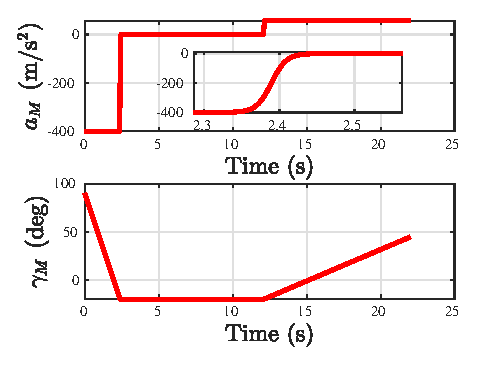
\includegraphics[width=\textwidth, keepaspectratio]{5_Images/amsigmakd.eps}
		\caption{Lateral acceleration $a_M(t)$ and flight path angle $\gamma_M(t)$.}
		\label{fig:ch_DP_sim1_accel}
	\end{subfigure}
	\caption{Target interception under TCT guidance with $\gamma_M(0) = 90^\circ$, desired approach angle $\theta_t = 45^\circ$, and terminal time $t^{\star} = 22.0\text{ s}$ ($r_d = 4,400\text{ m}$).}
	\label{fig:ch_DP_sim1_combined}
\end{figure}
\subsection{Arrival Time Variation via Design Radius $r_d$}

To demonstrate arrival time flexibility, Figure \ref{fig:ch_DP_sim2_radius_var} plots trajectories for a fixed approach angle $\theta_t = 45^\circ$ across varying design radii $r_d \in [r_m, r_{\text{crit}}^{\text{TCT}})$. Increasing $r_d$ expands the path length, smoothly shifting arrival times across $t_{\text{imp}} \in \{18.2\text{ s}, 22.0\text{ s}, 25.5\text{ s}\}$.

\begin{figure}[ht!]
	\centering
	\begin{subfigure}[b]{0.8\textwidth}
		\centering
		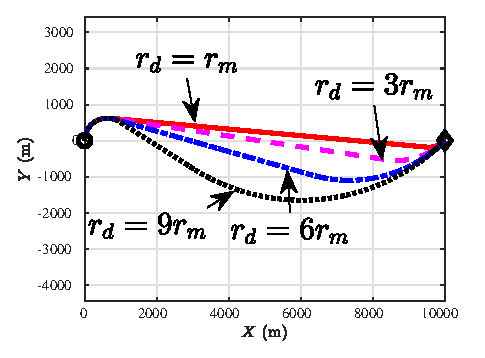
\includegraphics[width=\textwidth, keepaspectratio]{5_Images/traj_tct_compakd.eps}
		\caption{Trajectories for varying secondary radii $r_d$.}
		\label{fig:ch_DP_sim2_trajs}
	\end{subfigure}
	
	\vspace{1em}
	
	\begin{subfigure}[b]{0.8\textwidth}
		\centering
		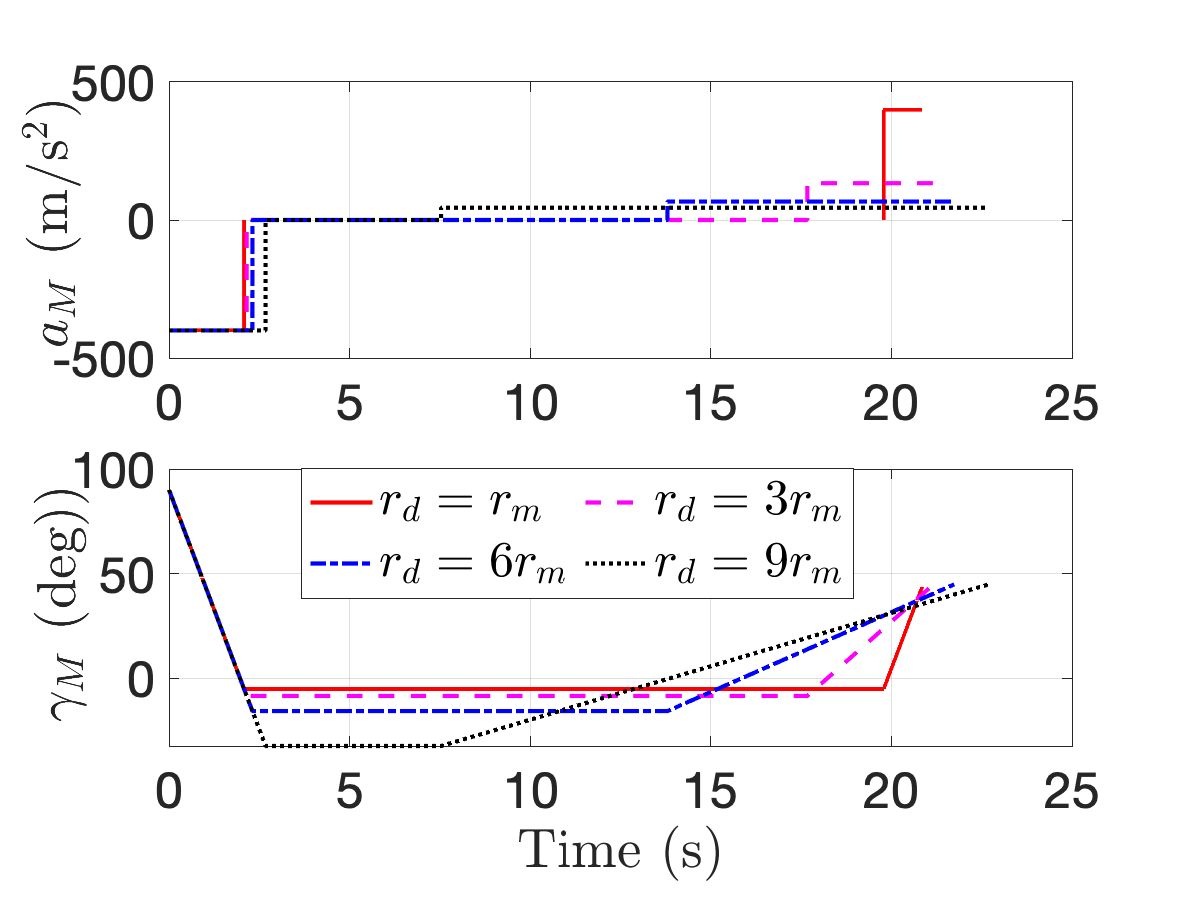
\includegraphics[width=\textwidth, keepaspectratio]{5_Images/amgammam_tct_compsrk.eps}
		\caption{Piecewise lateral acceleration profiles $a_M(t)$.}
		\label{fig:ch_DP_sim2_accel}
	\end{subfigure}
	\caption{Terminal arrival time tuning for $\theta_t = 45^\circ$ by adjusting secondary radius $r_d$.}
	\label{fig:ch_DP_sim2_radius_var}
\end{figure}

For extended arrival times ($t_{\text{imp}} \in \{60\text{ s}, 85\text{ s}, 100\text{ s}\}$), the mirrored TCT configuration ($C_2'$) is selected (Figure \ref{fig:ch_DP_sim3_outer}), validating unbounded arrival time capability.

\begin{figure}[ht!]
	\centering
	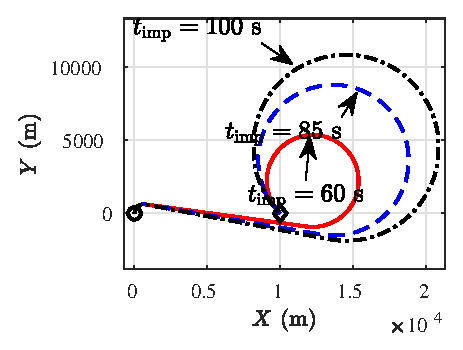
\includegraphics[width=0.85\textwidth, keepaspectratio]{5_Images/traj_out_tct1akd.eps}
	\caption{Large impact time trajectories ($t_{\text{imp}} \in \{60\text{ s}, 85\text{ s}, 100\text{ s}\}$) achieved using mirrored TCT geometry.}
	\label{fig:ch_DP_sim3_outer}
\end{figure}
\subsection{Comparative Evaluation with Existing Guidance Laws}
Figure \ref{fig:ch_DP_sim4_comparison} compares the proposed guidance protocol against two benchmark dual-constraint guidance laws: Zhang et al. \cite{Zhang2013} and Harl \& Willey \cite{harl2011impact}.

\begin{figure}[ht!]
	\centering
	\begin{subfigure}[b]{0.8\textwidth}
		\centering
		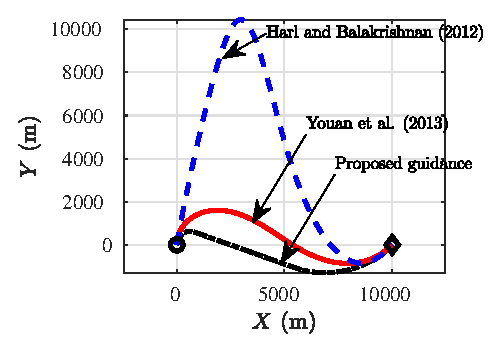
\includegraphics[width=\textwidth, keepaspectratio]{5_Images/traj_compakd.eps}
		\caption{Trajectory comparison.}
		\label{fig:ch_DP_sim4_trajs}
	\end{subfigure}
	
	\vspace{1em}
	
	\begin{subfigure}[b]{0.8\textwidth}
		\centering
		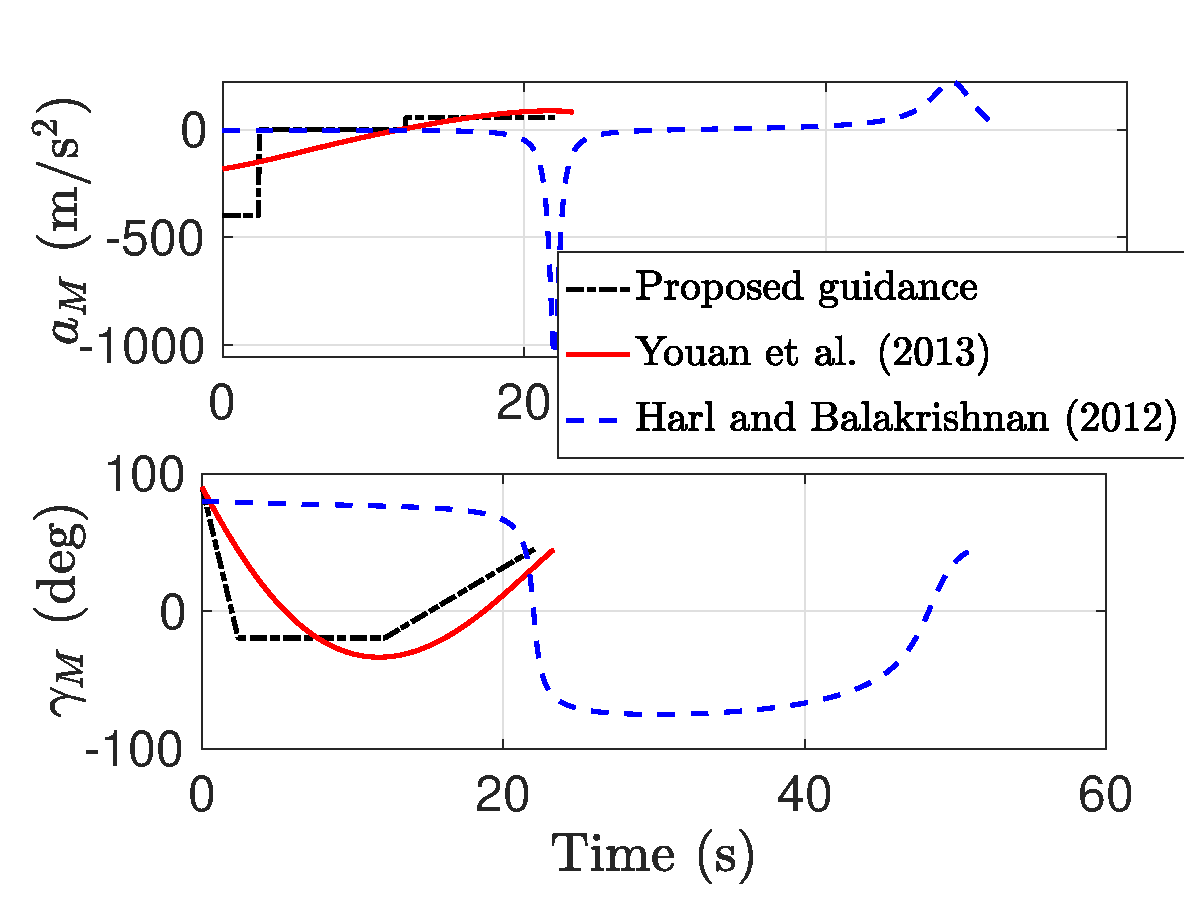
\includegraphics[width=\textwidth, keepaspectratio]{5_Images/am_comp_dubsrk.eps}
		\caption{Acceleration profile comparison.}
		\label{fig:ch_DP_sim4_accel}
	\end{subfigure}
	\caption{Performance comparison against existing guidance laws \cite{Zhang2013, harl2011impact} for $\theta_t = 45^\circ$ and $t^{\star} = 22.0\text{ s}$.}
	\label{fig:ch_DP_sim4_comparison}
\end{figure}
\begin{table}[ht!]
	\centering
	\caption{Comparative Guidance Performance Summary ($\theta_t = 45^\circ$, $t^{\star} = 22.0\text{ s}$)}
	\label{tab:ch_DP_comparison_table}
	\small
	\begin{tabularx}{\textwidth}{@{} >{\RaggedRight}X cccc @{}}
		\toprule
		\textbf{Guidance Method} & \textbf{Achieved } $t_{\text{imp}}$ \textbf{(s)} & \textbf{Achieved } $\theta_t$ & \textbf{Max } $|a_M|$ \textbf{(m/s}$^2$\textbf{)} & $\|a_M\|_1$ \textbf{(m/s}$^2$\textbf{)} \\
		\midrule
		Zhang et al. \cite{Zhang2013} & 23.35 & $45.0^\circ$ & 382.1 & 1,759.4 \\
		Harl \& Willey \cite{harl2011impact} ($\theta_M=80^\circ$) & 51.63 & $45.0^\circ$ & 400.0 & 2,401.9 \\
		\textbf{Proposed Dubins Protocol} & \textbf{22.00} & $\mathbf{45.0^\circ}$ & \textbf{400.0} & \textbf{1,517.3} \\
		\bottomrule
	\end{tabularx}
\end{table}
As summarized in Table \ref{tab:ch_DP_comparison_table}, Zhang's law \cite{Zhang2013} exceeds the desired arrival time ($23.35\text{ s}$ vs. $22.0\text{ s}$). Harl's law \cite{harl2011impact} singularizes at $\theta_M = 90^\circ$ and yields an erroneous arrival time of $51.63\text{ s}$ even when launched at $\theta_M = 80^\circ$. In contrast, the proposed Dubins protocol meets both terminal constraints precisely ($t_{\text{imp}} = 22.00\text{ s}, \theta_t = 45.0^\circ$) while consuming the lowest total acceleration energy ($\|a_M\|_1 = 1,517.3\text{ m/s}^2$).

\section{Summary}\label{sec:ch_DP_summary}
In this chapter, an open-loop and equivalent closed-loop trajectory planning framework was synthesized using Dubins-like path geometry to achieve simultaneous terminal approach angle $\theta_t$ and terminal arrival time $t_{\text{imp}}$ constraints against stationary targets. The primary conclusions are:
\begin{itemize}
    \item \textbf{Implementable Acceleration Profile:} The proposed guidance protocol demands piecewise-constant lateral acceleration across three discrete level acceleration profile ($+a^{\max}, 0, -a^{\max} \frac{r_m}{r_d}$), eliminating high-order polynomial computation and preventing actuator saturation.
    \item \textbf{Flexible Arrival Time Tuning:} Introducing variable secondary turn radius $r_d \ge r_m$ allows exact terminal time matching, while mirrored circle geometry ($C_2'$) renders achievable arrival times unbounded above.
    \item \textbf{Singularity-Free Closed-Loop Execution:} Distance-based closed-loop feedback \eqref{eq:ch_DP_closed_loop_guidance} with hyperbolic tangent smoothing removes trigonometric singularities at large lead angles ($\theta_M \approx 90^\circ$).
\end{itemize}

\vspace{0.5em}
\noindent %\textbf{Transition to Chapter 6:}\\
While Chapter \ref{ch:Dubins_Path} solved single-agent trajectory generation under nonholonomic constraints and terminal arrival time matching, coordinating multi-agent swarms in spatial pursuit scenarios requires integrating single-vehicle path geometry with collective team interception dynamics. 

Chapter \ref{ch:Spiral_Path} extends these geometric concepts to multi-agent swarm pursuit, formulating Archimedean spiral-based path synthesis and spatial rendezvous strategies for cooperative multi-interceptor teams.

%\chapter{Trajectory planning using Dubins-like paths with approach angle and terminal time constraints}\label{ch:5_Dubins_Path}









